\chapter{Descrizione della soluzione}
\label{chp:04-solution}
In questo capitolo verrà approfondito l'aspetto puramente pratico e le fasi che hanno portato alla realizzazione della soluzione; 
inoltre verranno mostrate le applicazioni pratiche degli aspetti teorici enunciati nei capitoli precedenti, unitamente alle difficoltà 
principali incontrate.

\section{Operazioni preliminari}
Prima di poter costruire il sistema di raccomandandazione proposto in questa tesi, sono state eseguite delle operazioni preliminari
per poter impostare il progetto di Django e la relativa applicazione che implementerà effettivamente la soluzione.\\

% TASSONOMIE E DATABASE CON I MODELS (package MPTT)
Come annunciato nei capitoli precendenti per procedere alla costruzione di un sistema di raccomandazione bisogna avere a disposizione
una base di dati solida da cui attingere tutte le informazioni; ed è proprio questo il primo passo che è stato seguito, disegnare 
e progettare una base di dati da cui partire per la realizzazione degli algoritmi proposti.
In generale Moon Cloud possiede una struttura delle Evaluation ad albero, quindi anche di conseguenza anche le tabelle del database 
rispecchiano questa struttura, sulla base delle considerazioni sulle tecniche adottate sono state fatte nei capitoli precendenti.\\
Per implementare un modified pre-order trasversal tree in Django, si è fatto uso del package MPTT, come detto in precendenza, questa
tecnica è usata per memorizzare dati gerarchici in un database, puntando all'efficenza nelle operazioni di recupero dei dati e 
scendendo a compromessi per quanto riguarda le operazioni di inserimento e spostamento dei nodi all'interno della struttura.
Grazie all'usilio di questa utility la costruzione dei Model del progetto sono stati semplificati e qui di seguito \ref{lst:models}
è possibile trovare le porzioni principali del codice costituente i Model, i quali poi vengono utilizzati da Django per la 
generazione della base di dati. 

% MODELS CODES
\lstset{style=python_code_style}
\label{lst:models}
\begin{lstlisting}[language=Python, caption={Parti principali del codice dei Models della soluzione}]
# Target supported by Moon Cloud
class TargetType(models.Model):
	TYPES = (
		('host', 'host'),
		('windows', 'windows'),
		('url', 'url'),
		('azure', 'azure'),
		('aws', 'aws')
	)
	name = models.CharField(max_length=150, choices=TYPES, default="host")
	descr = models.TextField(max_length=1000, default="none")  # Description of a targe


# Control that can be part of evaluations
class Control(MPTTModel):
	other_id = models.IntegerField(default=-1, unique=True)
	parent = TreeForeignKey('self', on_delete=models.CASCADE, null=True, blank=True, related_name='children')
	name = models.CharField(max_length=150, unique=True)
	descr = models.TextField(max_length=1000, default="none")  # Description of a node in the taxonomy
	TYPES = (
		('cat', 'category'),
		('con', 'control')
	)
	# Possible node type of the taxonomy (category node or control node)
	node_type = models.CharField(max_length=3, choices=TYPES, default='cat')
	target_type = models.ForeignKey(TargetType, null=True, blank=True, on_delete=models.CASCADE)  # It's null for the root node and category nodes


# Evaluation used by users (group of controls)
class Evaluation(MPTTModel):
	other_id = models.IntegerField(default=-1, unique=True)
	parent = TreeForeignKey('self', on_delete=models.CASCADE, null=True, blank=True, related_name='children')
	name = models.CharField(max_length=150, unique=True)
	descr = models.TextField(max_length=1000, default="none")  # Description of a node in the taxonomy
	TYPES = (
		('cat', 'category'),
		('eva', 'evaluation')
	)
	# Possible node types of the taxonomy (category node or evaluation node)
	node_type = models.CharField(max_length=3, choices=TYPES, default='cat')
	controls = models.ManyToManyField(Control)  # Evaluation can be composed of one or more controls


# Users with a Moon Cloud account who can use evaluations
class User(models.Model):
	other_id = models.IntegerField(default=-1, unique=True)
	email = models.EmailField(max_length=50, unique=True)
	evaluations = models.ManyToManyField(Evaluation, blank=True)  # Evaluations chosen by user


# Target table to save the targets type (more than one) that a user can have
class Target(models.Model):
	user = models.ForeignKey(User, blank=True, on_delete=models.CASCADE)  # User has chosen some target_type
	other_id = models.IntegerField(default=-1, unique=True)
	target_type = models.ForeignKey(TargetType, blank=True, on_delete=models.CASCADE)  # TargetType Id
\end{lstlisting}


A partire da questo Model vennero introdotte nel database le seguenti tabelle, le quali è possibile visionare nella Figura 
\ref{fig:str_db_project}:
\begin{description}
	\item[Control]: contiene l'insieme dei software che vengono poi effetivamente eseguiti all'interno di una Evaluation, 
	i campi other\_id (identificativo che fa riferimento al database effetivo di Moon Cloud),
	descr (una descrizione del funzionamento del controllo), node\_type (definisce se il nodo è un Evaluation o un nodo Categoria)
	definiscono le caratteristiche del controllo mentre lft, rght, tree\_id, level e parent sono introdotti 
	automaticamente dal package MPTT per poter rappresentare i dati in modo gerarchico, infine target\_type\_id rappresenta, quel
	controllo a quale Target viene associato. 
	\item[Evaluation]: contiene l'insieme di Evaluation che un utente può eseguire per un certo Target, e allo stesso modo 
	i campi contenuti nella tabella Control. La tabella intermedia evaluation\_controls permette di memorizzare quali controlli
	sono associati a quali Evaluation.
	\item[User]: contiene gli utenti registrati alla piattaforma Moon Cloud, e sono anche loro, come con le tabelle precedenti,
	identificati con un campo other\_id, e distinti da un email. La tabella intermedia user\_evaluations permette di memorizzare 
	quali Evaluation un utente ha selezionato e usato.
	\item[Target]: è utilizzata per memorizzare quali Target un utente ha inserito e sui quali vuole effettuare dei processi
	di Evaluation.  
	\item[TargetType]: specifica quali sono i tipi di Target supportati da Moon Cloud.
\end{description}

\begin{figure}[ht!]
	\centering
	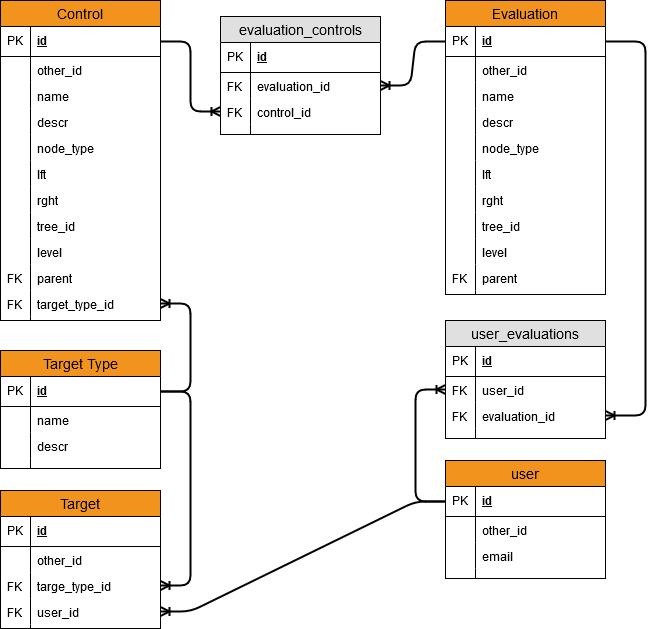
\includegraphics[scale=0.7]{images/MoonCloudRecommendation_ER.png}
	\caption{Struttura del database}
	\label{fig:str_db_project}
\end{figure}





% ASPETTI DI DJANGO CHE HO PERSONALIZZATO, COME LE ADMIN PAGE

% URLS e VIEW A SCOPO DIDATTICO

% VIEW PER LE RACCOMANDAZIONI

% VIEW PER MANTERE LA CONSISTENZA COL MIO DATABASE

% IMPLEMENTAZIONE CON DOCKER

